\chapter{Task 15 - SOC and Cascade Optimization in Coupled Sandpiles}
\label{ch:task15}

\section{Theoretical Introduction}

The primary objective of this investigation is to identify the optimal interconnectivity threshold that minimizes global risk in coupled infrastructures, balancing the trade-offs that govern cascades of load shedding.\cite{brummitt2012suppressing} While establishing links between independent networks allows a critical system to initially divert excess load to a neighboring module acting as a reservoir, excessive coupling paradoxically accelerates systemic vulnerability by opening open pathways for destructive, cross-module cascade propagation.\cite{brummitt2012suppressing} To quantitatively evaluate these dynamics, the \textbf{Bak-Tang-Wiesenfeld (BTW)} sandpile formulation is simulated on a multitype network framework composed of two interacting modules, $A$ and $B$, generated via a regular configuration model where each node possesses an identical internal degree $z_a = z_b = 3$ and a total system size of $N = 2000$ vertices per module.\cite{brummitt2012suppressing}

The driving mechanism introduces units of load stochastically and uniformly across the nodes.\cite{brummitt2012suppressing} Every vertex $i$ is characterized by an innate capacity threshold equal to its total degree $k_i$.\cite{brummitt2012suppressing} Whenever the accumulated load $h_i$ strictly exceeds this capacity, the node becomes unstable and undergoes a shedding event, transferring exactly one unit of load to each of its $k_i$ neighbors.\cite{brummitt2012suppressing} The balancing transport equation governing the redistribution of load from a triggered node $i$ to its adjacent neighborhood $\mathcal{N}(i)$ is formulated as:\cite{bak1987self}

\begin{equation}\label{eq:load_shedding_flow}
    \begin{cases}
        h_i \longrightarrow h_i - k_i \\
        h_j \longrightarrow h_j + 1 & \forall \, j \in \mathcal{N}(i)
    \end{cases}
\end{equation}

To establish a stationary critical state and avoid indefinite mass accumulation on finite graphs, a uniform dissipation rate $f$ is integrated into the propagation rule.\cite{brummitt2012suppressing} During each shedding event, individual grains are independently deleted from the system with a small probability $f$ as they traverse the links, effectively controlling the characteristic exponential cutoff scale of the largest global cascades.\cite{brummitt2012suppressing}

\newpage

\section{Network Topology and Simulation Setup}

The modular topology is assembled by implementing a Bernoulli-distributed coupling mechanism to establish sparse interdependencies between the regular baselines.\cite{brummitt2012suppressing} Under this multitype configuration, each node in module $A$ receives exactly one external edge stub with a coupling probability $p$, and zero stubs with probability $1-p$.\cite{brummitt2012suppressing} These external stubs are subsequently matched and wired uniformly at random with a corresponding sequence of stubs generated independently in module $B$.\cite{brummitt2012suppressing} From a structural standpoint, the creation of an inter-module bridge increments both the local degree $k_i$ and the capacity threshold of the endpoint vertex by one unit.\cite{brummitt2012suppressing}

The numerical analysis explores the transition from microscopic stochastic events to macroscopic collective vulnerabilities by testing how the network interconnection alters the total cascade distribution profiles.\cite{brummitt2012suppressing} The statistics of the cascading events are evaluated using the complementary cumulative distribution function (CCDF), which filters out statistical noise in the distribution tails. Figure~\ref{fig:microscopic_avalanche_distributions} outlines the microscopic properties of the cascade ensembles recorded over $5 \times 10^5$ driving steps after discarding a transient loading phase of $5 \times 10^4$ steps.

\begin{figure}[htbp]
    \centering
    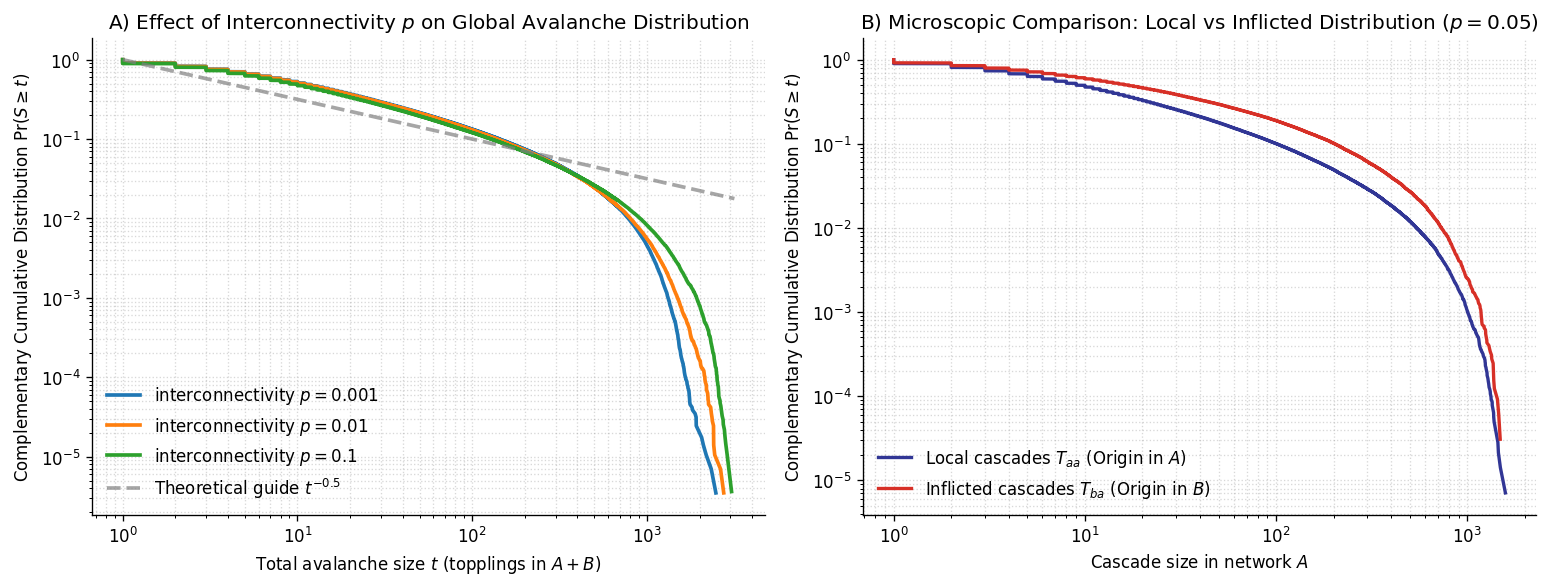
\includegraphics[width=0.95\textwidth]{images/plot1.png}
    \caption{(Left) CCDF log-log distribution of the total cascade size $t$ ($A+B$) for three coupling regimes ($p=0.001, 0.01, 0.1$), compared against the mean-field scaling guide $t^{-0.5}$. (Right) Microscopic comparison between the localized cascade sizes $T_{aa}$ (origin in $A$) and the exogenous inflicted cascades $T_{ba}$ (origin in $B$) at a fixed coupling level $p=0.05$.}
    \label{fig:microscopic_avalanche_distributions}
\end{figure}

For intermediate scaling windows, the empirical data match the classic mean-field power-law exponent ($\tau = 3/2$, implying a CCDF slope of $-0.5$) typical of sparse, locally tree-like random regular topologies where the branching process approximation becomes exact.\cite{brummitt2012suppressing, goh2003sandpile} As the interconnectivity $p$ increases from $0.001$ to $0.1$, the total available capacity scales up, shifting the exponential cutoff toward larger cascade sizes $t$ and enabling system-wide global propagation.\cite{brummitt2012suppressing} Isolating the directional flow of risk at $p = 0.05$, the distribution tail of the inflicted cascades ($T_{ba}$) decays slower than that of the purely local events ($T_{aa}$).\cite{brummitt2012suppressing} This diagnostics validates the structural role of inter-module bridges, which act as efficient conduits for cross-module load transfer, amplifying external load shocks.\cite{brummitt2012suppressing}

\section{Macroscopic Phase Space and Stability}

Integrating the statistical event counts, the systemic risk is projected onto a macroscopic phase space to trace the emergence of an optimal network topology.\cite{brummitt2012suppressing} A large cascade is defined via a threshold cutoff $C = N/2 = 1000$ nodes.\cite{brummitt2012suppressing}

\begin{figure}[htbp]
    \centering
    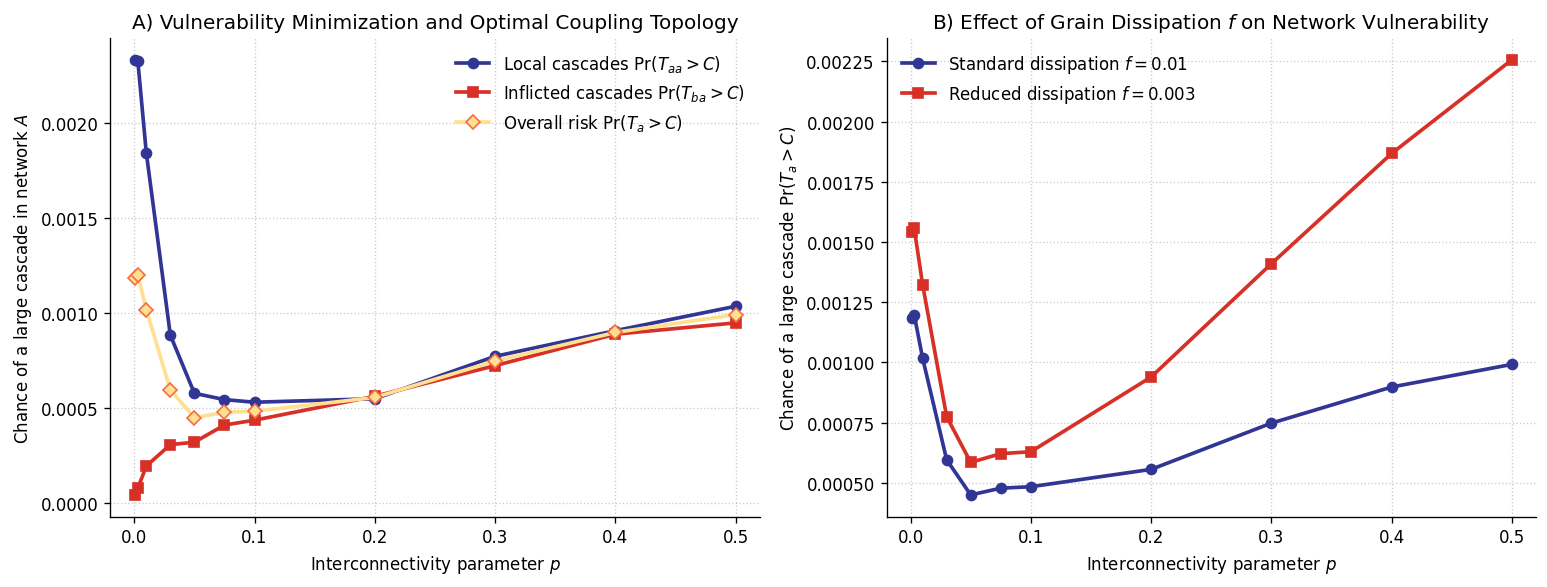
\includegraphics[width=0.95\textwidth]{images/plot2.png}
    \caption{(Left) Linear phase space of the large cascade probabilities ($\Pr(T > 1000)$) as a function of the interconnectivity $p$, highlighting the decomposition into local, inflicted, and overall risk. (Right) Sensitivity analysis illustrating the overall cascading risk profile under standard ($f=0.01$) and reduced ($f=0.003$) grain dissipation.}
    \label{fig:macroscopic_phase_space}
\end{figure}

The linear phase space outlined in Figure~\ref{fig:macroscopic_phase_space} maps a non-monotonic vulnerability profile.\cite{brummitt2012suppressing} At small $p$, increasing the number of bridges suppresses local cascades ($\Pr(T_{aa} > C)$ drops) because the neighboring network acts as a dissipating reservoir that absorbs excess load.\cite{brummitt2012suppressing} Conversely, at high $p$, strong coupling increases capacity and enables inflicted cascades ($\Pr(T_{ba} > C)$ rises), letting fluctuations return with catastrophic effects.\cite{brummitt2012suppressing} To extract the continuous minimum independent of the discrete grid points, a local second-degree polynomial windowing is applied within the sella region ($p \in [0.01, 0.15]$), yielding an optimal coupling point at $p^* \approx 0.0717$, in agreement with the analytical predictions ($0.075 \pm 0.01$).\cite{brummitt2012suppressing}

A sensitivity analysis checks the structural vulnerability of the phase space against changes in the conservation rules. Under a reduced dissipation rate ($f = 0.003$), the system retains a larger mass fraction per shedding event.\cite{brummitt2012suppressing} The entire vulnerability profile undergoes a vertical translation, amplifying the frequency of large events and accelerating the catastrophic risk ascent at high $p$, while preserving the geometric localization of the optimal coupling minimum.\cite{brummitt2012suppressing}